\RequirePackage{plautopatch}

\documentclass[uplatex,dvipdfmx]{jsarticle}

\usepackage{amsmath, amsthm}
\usepackage{url}
\usepackage[dvipdfmx]{graphicx}
\usepackage[normalem]{ulem}
\usepackage[utf8]{inputenc}
\usepackage{hyperref}
\usepackage{biblatex}

\addbibresource{bib_logo_tsuokay.bib}

\renewcommand{\figurename}{Fig.} %図のキャプションをFig.〇にする
\renewcommand{\tablename}{Table } %表のキャプションをTable 〇にする
\setcounter{tocdepth}{3} %\subsubsectionまで目次に表示する

\begin{document}

\begin{titlepage}
  \noindent %段落の文字下げ防ぐ
  \\ \\ \\ \\ \\ \\ \\ \\ 
  \begin{center}
  \begin{LARGE}
  
    研究室のロゴ作成のログ

  \end{LARGE}
  \end{center}
  \vspace{7cm}
  \begin{center}
  \begin{LARGE}
  岡山 毅\\
  tsuyoshi.okayama@gmail.com
  \end{LARGE}
  \end{center}
  % \markright{ver.2023.03.09} 
\end{titlepage}
\newpage

\tableofcontents
\newpage

\section{本プロジェクトの概要}

4Dは大事である\cite{Schunck2021}。

現段階(2023.06.05)時点での研究室名は"Agri3(Agri-cubed) lab"である。この研究室名を3次元で表現し、アニメーションを作成したい。同時にHoudiniの技術的な訓練も兼ねる。

現時点で考えている手順は以下の通り。適宜、用語についてはCG用言語として適切なものに変更していくこと。

\bigskip
\begin{itemize}
  \item 3次元文字を表示する
  \item 文字を立体的にする
  \item カメラ位置を設定する
  \item レンダリングをする
  \item "3"の数字から光を出す
  \item "3"の数字を移動させる
  \item "Agri"についての工夫をこらす
\end{itemize}


\section{2023.06.06の作業}
"polyExtrude"を使用して、文字を立体化。
standard materialsを使ってレンダリングしてみる。成果はこれ Fig. \ref{fig:rendered_230606}。


\begin{figure}[h]
  \centering
  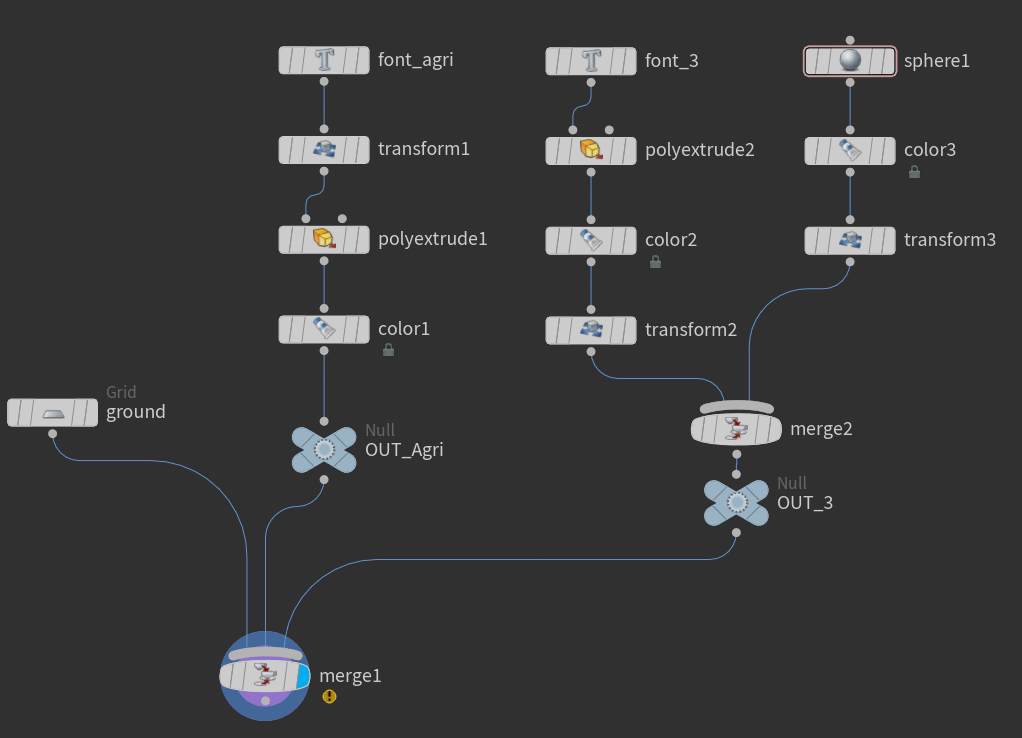
\includegraphics[width=0.7\textwidth]{figs/network_230606.PNG}
  \caption{2023.06.06のネットワーク}
  \label{fig:network_230606}
\end{figure}

しかし奥が深い。

\bigskip
改善項目
\begin{itemize}
  \item 全体的に暗い
  \item 球は光らすのではないのか
  \item "Agri"はこのように単純で良いのか
\end{itemize}

\begin{figure}[h]
  \centering
  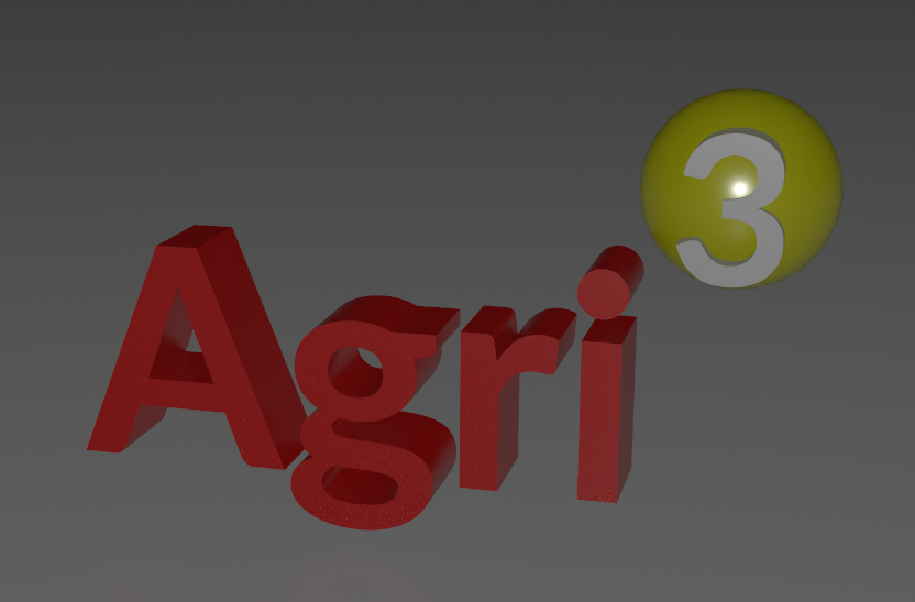
\includegraphics[width=0.7\textwidth]{figs/logo_230606.PNG}
  \caption{2023.06.06のレンダリング結果}
  \label{fig:rendered_230606}
\end{figure}


\subsection{球を発光させる}
geometoryを分ける必要がありそう\footnote{理論と実践で学ぶHoudini P622}。

球を別のgeometryで作成し、Lights and CamerasのGeometry lightを選択してみる。

\begin{figure}[h]
  \centering
  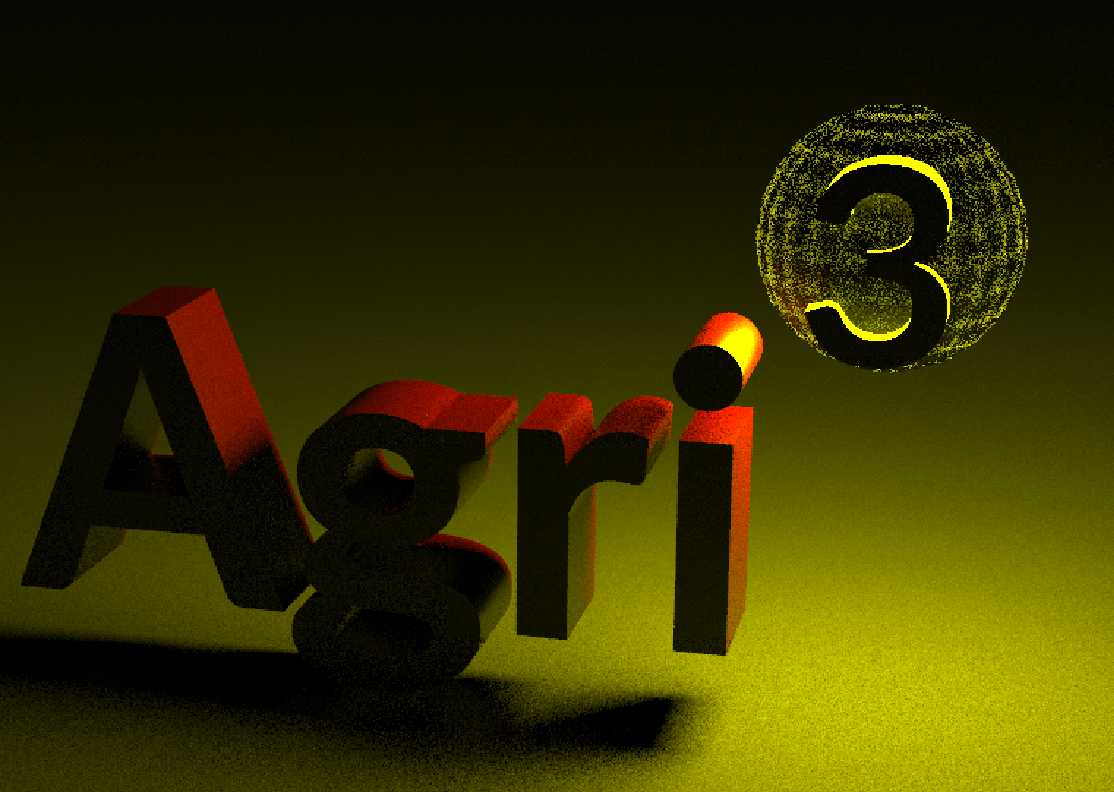
\includegraphics[width=0.7\textwidth]{figs/fig_light_3.PNG}
  \caption{2023.06.06のレンダリング結果}
  \label{fig:rendered_230606_2}
\end{figure}


立体にした途端に、重力が無いように見えて違和感がでるのが面白い。
どういうことだろうか。fig \ref{fig:rendered_230606_2}とfig. \ref{fig:rendered_230606_3}の違いがよくわからない。発光についての知識も不足している。

\begin{figure}[h]
  \centering
  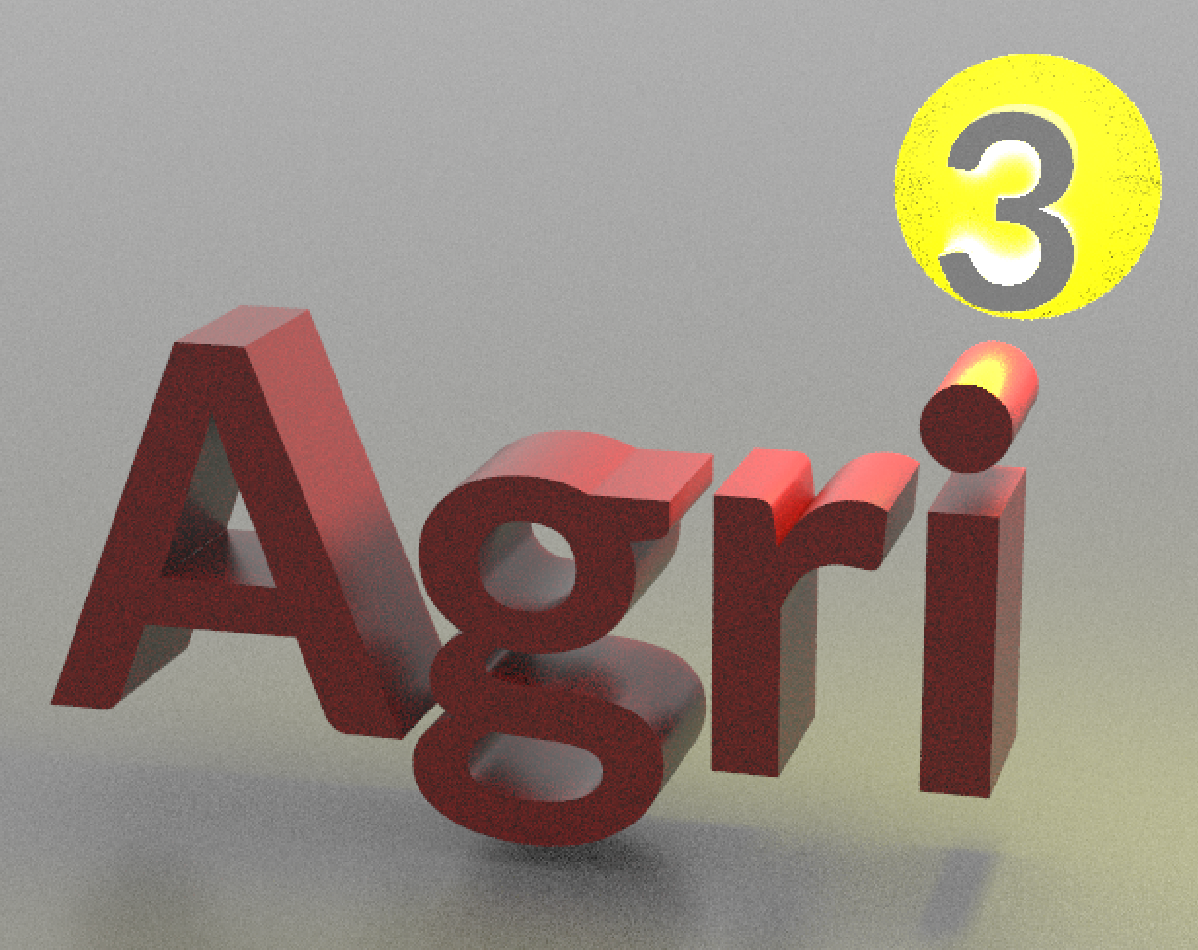
\includegraphics[width=0.7\textwidth]{figs/fig_light_4.PNG}
  \caption{2023.06.06のレンダリング結果}
  \label{fig:rendered_230606_3}
\end{figure}

\printbibliography

\end{document}